\section{Технический проект}
\subsection{Общая характеристика организации решения задачи}

Для реализации поставленных задач необходимо спроектировать и разработать программно-информационную систему, включающую в себя десктопное приложение с интерфейсом для взаимодействия с базой данных.

Ключевой особенностью архитектуры системы является её модульность — каждый компонент может быть адаптирован, масштабирован или заменён без нарушения работы остальных частей. Пользователь взаимодействует с графическим интерфейсом, формируя запросы к встроенной базе данных. Внутренняя реализация позволяет использовать в качестве интерфейса командный синтаксис, аналогичный SQL, с поддержкой типизации, условий, фильтрации и логических операций.

Программа ориентирована на использование в условиях, когда установка полноценных СУБД невозможна или избыточна: в образовательных целях, на встраиваемых устройствах, в изолированных системах и во временных проектах. При этом поддержка сериализации и сохранения баз данных на диск обеспечивает сохранность данных между сессиями.

Основной акцент при проектировании сделан на простоту взаимодействия, прозрачную структуру хранения данных, а также модульную реализацию команд, что упрощает тестирование и расширение функциональности.

\subsection{Обоснование выбора технологии проектирования}

Выбор технологий, языков программирования и архитектурных решений для реализации программно-информационной системы обусловлен совокупностью факторов, направленных на обеспечение высокой гибкости, надёжности и простоты сопровождения программного продукта. Используемые для создания программно-информационной системы языки и технологии отвечают современным практикам разработки, позволяют достичь высокой производительности и отказоустойчивости программы.

\subsubsection{Язык программирования Python}

В качестве основного языка программирования выбран Python, благодаря его сочетанию выразительности, гибкости и обширной поддержки со стороны сообщества разработчиков. Python — это высокоуровневый, интерпретируемый язык, активно применяющийся как в образовательных, так и в промышленных проектах. Основные причины выбора языка заключаются в следующем:
\begin{enumerate}
	\item Простой и интуитивно понятный синтаксис значительно сокращает порог вхождения и снижает количество потенциальных ошибок при написании кода. Это особенно важно в условиях ограниченного времени на разработку и тестирование, а также при передаче проекта на сопровождение.
	\item Поддержка нескольких парадигм программирования, включая объектно-ориентированную, процедурную и функциональную, делает Python универсальным инструментом. Это позволяет организовать код в соответствии с принципами модульности, инкапсуляции и повторного использования.
	\item Обширная стандартная библиотека и внешняя экосистема обеспечивают доступ к готовым модулям для сериализации, построения интерфейса, анализа синтаксических деревьев, многопоточности и многого другого. Это существенно ускоряет разработку и упрощает реализацию сложных функций.
	\item Кроссплатформенность языка позволяет запускать приложение на операционных системах Windows, Linux и macOS без необходимости адаптации кода под конкретную платформу. Таким образом, обеспечивается максимальная универсальность и доступность системы для пользователя.	
\end{enumerate}
Таким образом, Python представляет собой оптимальное решение для реализации проекта, сочетающее в себе простоту, мощь и гибкость, что делает его незаменимым инструментом в учебных и практических задачах программной инженерии.

\subsubsection{Графический интерфейс с использованием tkinter}

Для построения графического интерфейса выбрана библиотека tkinter, являющаяся частью стандартной поставки Python и представляющая собой обёртку над библиотекой Tcl/Tk. Выбор данного инструмента объясняется рядом технологических и практических преимуществ:
\begin{enumerate}
	\item Отсутствие необходимости в установке сторонних зависимостей делает tkinter особенно удобным для использования в проектах с упрощённым процессом развёртывания. Пользователь может сразу запустить приложение без дополнительных установок, что критично в условиях учебной и демонстрационной среды.
	\item Простота проектирования интерфейса позволяет легко создавать окна, формы, кнопки, меню, вкладки и другие элементы, без необходимости изучения сложных графических фреймворков. Это обеспечивает быстрое создание прототипов и конечного интерфейса.
	\item Полная кроссплатформенность интерфейса обеспечивает его одинаковое отображение и поведение на всех операционных системах, что избавляет разработчика от необходимости писать отдельные реализации под разные платформы.
	\item Наличие компонентов высокого уровня, таких как текстовые поля, выпадающие списки, кнопки, панели и таблицы, позволяет создать функциональный и интуитивно понятный интерфейс для работы с базой данных.
	\item Возможность динамического обновления интерфейса обеспечивает удобную визуализацию изменений в таблицах, реализацию фильтрации, командных операций и навигации по вкладкам с таблицами.
\end{enumerate}

Tkinter полностью удовлетворяет требованиям к простому, лёгкому в использовании, но функциональному графическому интерфейсу.

\subsubsection{Обработка выражений с использованием ast}

Обработка пользовательских условий в командах select, update, delete реализована с использованием модуля ast, предоставляющего средства для разбора и анализа абстрактного синтаксического дерева Python-кода. Преимущества данного подхода включают:
\begin{enumerate}
	\item Безопасность: использование ast обеспечивает безопасную альтернативу функции eval, так как исключает возможность выполнения произвольного и потенциально вредоносного кода. Все выражения анализируются на уровне структуры, без исполнения.
	\item Гибкость: дерево выражения можно программно обойти и обработать только допустимые узлы, игнорируя и блокируя потенциально опасные конструкции, такие как вызовы функций или импорты.
	\item Контролируемость и расширяемость: при необходимости можно легко расширить список допустимых операций или добавить поддержку новых выражений. 
	\item Производительность: несмотря на дополнительную стадию разбора, использование ast не создаёт ощутимой нагрузки на систему, благодаря высокой скорости работы с синтаксическими деревьями.
\end{enumerate}

\subsubsection{Сериализация и хранение с использованием pickle}

Для хранения базы данных используется механизм сериализации объектов с помощью модуля pickle, который входит в стандартную библиотеку Python. Преимущества такого подхода:
\begin{enumerate}
	\item Универсальность: pickle способен сериализовать практически любые структуры данных Python, включая вложенные списки, словари, экземпляры пользовательских классов и даже функции. Это позволяет сохранить всю структуру базы данных и состояние приложения без дополнительной обработки.
	\item Простота реализации: сериализация и десериализация данных осуществляются в несколько строк кода, что упрощает поддержку и снижает вероятность ошибок. В рамках проекта реализовано автоматическое сохранение базы при закрытии и восстановление при запуске.
	\item Высокая скорость: по сравнению с текстовыми форматами хранения (например, CSV или JSON), бинарный формат pickle обеспечивает более быстрое чтение и запись, что особенно важно при работе с большими объёмами данных.
	\item Портируемость: сериализованные файлы можно переносить между машинами, при условии совпадения версий Python и структуры классов, что позволяет легко мигрировать проект или создавать резервные копии.
\end{enumerate}

\subsection{Архитектура программной системы}

Архитектура программно-информационной системы спроектирована с приоритетом на модульность, расширяемость и независимость компонентов, что позволяет обеспечивать как простоту разработки, так и готовность к дальнейшему масштабированию. Такое решение особенно актуально в условиях ограниченных ресурсов, когда необходимо добиться максимальной функциональности при минимальных затратах времени и вычислительных ресурсов.

\subsubsection{Общая структура системы}

Программа условно разделена на три основных логических уровня:
\begin{enumerate}
	\item Логическое ядро — реализует логику обработки команд, взаимодействие с внутренним представлением базы данных, интерпретацию пользовательского ввода и выполнение операций (select, insert, delete, update и др.).
	\item Графическая оболочка — отвечает за взаимодействие с пользователем через визуальный интерфейс, реализованный с использованием библиотеки tkinter.
	\item Модуль хранения и сериализации — обеспечивает сохранение состояния базы данных в бинарном виде и восстановление при запуске программы с использованием стандартного модуля pickle.
\end{enumerate}

Такое многоуровневое разбиение позволяет выполнять независимую разработку, модификацию и тестирование каждого из компонентов, не затрагивая остальную часть системы.

\subsubsection{Модульность и принципы проектирования}

Основу архитектурного подхода составляют принципы разделения ответственности, низкой связанности, повторного использования и тестируемости.

Разделение ответственности — каждый компонент системы выполняет строго определённую функцию: ядро не знает о графике, графика не взаимодействует напрямую с файлами хранения, и т.д.

Низкая связанность — компоненты взаимодействуют друг с другом через чётко определённые интерфейсы, что позволяет при необходимости заменить реализацию одного из модулей без необходимости переписывания остальной части приложения.

Повторное использование — логическое ядро оформлено в виде отдельного модуля Python, что позволяет импортировать его в других проектах как библиотеку, использовать в скриптах автоматизации или интегрировать в другие пользовательские интерфейсы.

Тестируемость — благодаря изоляции логики от графики, функциональность ядра может быть протестирована с использованием модульных тестов, без запуска графической части. Это повышает надёжность программы и упрощает отладку.

\subsubsection{Поток выполнения и взаимодействие компонентов}

Система построена по модульной архитектуре с явным разделением ответственности между компонентами. Все модули взаимодействуют по иерархии "<сверху вниз">:
\begin{enumerate}
	\item Пользователь взаимодействует с приложением через графическую оболочку. Эта оболочка содержит обработчики событий, виджеты (таблицу, формы, кнопки, поле ввода) и элементы навигации.
	\item Графическая оболочка передаёт все команды и параметры непосредственно в логическое ядро, которое выступает в роли контроллера и интерпретатора команд.
	\item Логическое ядро реализует	интерпретацию пользовательских команд (анализ строк, парсинг); обработку условий через ast; реализацию операций с таблицами: фильтрацию, выборку, обновление, удаление, сортировку и т.п.; валидацию данных и логических ошибок. При этом ядро не зависит от графической оболочки и может использоваться отдельно (например, в консольном режиме или как внешняя библиотека).
	\item Вся информация хранится в внутренней модели данных, которая представляет таблицы как структуры на основе словарей и списков. Модель полностью находится в оперативной памяти во время работы программы.
	\item Для долговременного хранения используется модуль сериализации, основанный на pickle. Он обеспечивает сохранение всей модели данных в бинарный файл при выходе из приложения и её восстановление при следующем запуске.
\end{enumerate}

\subsection{Архитектура десктопного приложения}

Точкой входа в программу является модуль main.py, в котором создаётся и запускается экземпляр класса MainWindow, реализующего основной графический интерфейс приложения. Архитектура построена с приоритетом на модульность и разделение ответственности, что облегчает поддержку, тестирование и возможное расширение проекта.

Архитектура приложения состоит из следующих ключевых модулей:
\begin{enumerate}
	\item main.py — стартовый модуль, в котором производится инициализация пользовательского интерфейса. Здесь создаётся объект MainWindow, который затем запускается методом mainloop(). Этот файл минимален по содержанию и служит точкой входа в приложение.
	\item dbwindow.py — содержит основной класс пользовательского интерфейса MainWindow, реализованный с использованием библиотеки tkinter. Класс отвечает за построение структуры окна, создание вкладок для различных таблиц, отображение командной панели, визуальных фильтров, меню и таблиц. Взаимодействие с моделью данных и логическим ядром осуществляется через внутренние методы и обработчики событий. Все элементы интерфейса организованы по принципу событийного программирования.
	\item database.py — реализует класс Database, представляющий собой структуру хранения данных. Он содержит таблицы в виде словарей и предоставляет методы добавления, удаления, выборки и сериализации данных. Класс инкапсулирует взаимодействие с файловой системой (через pickle) и отвечает за сохранность и восстановление состояния при запуске/выходе из программы.
	\item table.py — содержит реализацию класса Table, представляющего одну таблицу базы данных. Класс обеспечивает работу с полями и строками, а также поддерживает базовые операции (insert, delete, update, select), реализуемые как на уровне структуры, так и логически. Этот класс тесно взаимодействует с логическим ядром, обеспечивая доступ к данным.
	\item parser.py — содержит логическое ядро системы: функции parse\_command и eval\_node. Этот модуль обрабатывает команды пользователя, разбирая их в абстрактное синтаксическое дерево с помощью модуля ast и интерпретируя выражения. Таким образом реализуется внутренняя система команд, имитирующая простейший SQL-язык. Здесь выполняется обработка условий в командах select, update и delete посредством функции eval\_node. Модуль работает независимо от интерфейса и может использоваться повторно в других системах.
\end{enumerate}

Компоненты приложения взаимодействуют по следующему принципу:
\begin{enumerate}
	\item Интерфейс (класс MainWindow) получает команды пользователя, введённые в поле ввода и передаёт их в parser.py на обработку.
	\item parser.py анализирует синтаксис команды, выполняет преобразование и обращается к объекту Database, который, в свою очередь, обращается к хранящимся внутри него объектам Table, которые выполняют соответствующие действия с данными.
	\item Изменения в модели данных отражаются в интерфейсе: таблицы обновляются, состояние базы сохраняется.
	\item Сохранение и загрузка базы реализованы через сериализацию: объект Database сохраняется в бинарный файл с использованием pickle, обеспечивая простоту и надёжность хранения.
\end{enumerate}

Между компонентами минимально необходимая связь: GUI не содержит логики обработки выражений, а ядро не зависит от визуального представления. Это упрощает поддержку, тестирование и потенциальную адаптацию под другие платформы.

Архитектура гибкая, расширяемая и легко масштабируемая — возможно добавление новых типов команд, а также подключение внешних источников данных или API без необходимости переписывания основной логики.

\subsection{Проект данных программной системы}

Исходя из требований технического задания, программно-информационная система предназначена для работы с пользовательскими табличными структурами, которые хранятся в оперативной памяти и при необходимости сохраняются на диск. Система не использует сторонние серверные СУБД, а реализует собственную модель хранения и управления данными средствами языка Python.

Для организации хранения данных в системе разработана внутренняя структура, состоящая из двух основных компонентов: база данных и таблица. Каждая база данных представлена отдельным файлом с расширением .db, содержащим сериализованное состояние всех таблиц. Сохранение и загрузка данных осуществляется с помощью стандартной библиотеки pickle, позволяющей преобразовывать объекты Python в бинарный формат и обратно.

\subsubsection{Структура данных}

Каждая база данных содержит произвольное количество таблиц. Таблица обладает уникальным именем и определённой схемой, включающей набор столбцов с заранее определёнными типами данных. В системе поддерживаются три типа данных:
\begin{itemize}
	\item integer -- целочисленные значения, соответствующие типу int в Python;
	\item float -- числа с плавающей точкой -- float;
	\item string -- строковые значения (str).
\end{itemize}

Система строго соблюдает типизацию: при вставке и обновлении строк выполняется проверка соответствия типов в каждой ячейке данным, указанным в схеме таблицы. Нарушение соответствия приводит к отклонению команды и выводу сообщения об ошибке.

Внутреннее представление таблицы реализовано как структура данных, содержащая:
\begin{itemize}
	\item список названий столбцов;	
	\item словарь, сопоставляющий имя столбца и его тип;	
	\item список строк. Каждая строка -- это словарь значений, где ключи -- названия столбцов, а значения -- данные соответствующего типа.
\end{itemize}

Данные в таблице могут быть изменены при помощи четырёх базовых операций:
\begin{itemize}
	\item insert — вставка новой строки;	
	\item select — выборка строк с фильтрацией по условиям;	
	\item update — обновление значений в строках, удовлетворяющих заданному условию;	
	\item delete — удаление строк.
\end{itemize}

\subsubsection{Хранение и сериализация}

Все таблицы базы данных сохраняются в файл с помощью модуля pickle. Хранение происходит в бинарном формате, позволяющем без дополнительных преобразований сериализовать сложные структуры: списки, словари, экземпляры классов и пр. Такой подход обеспечивает следующие преимущества:
\begin{itemize}
	\item отсутствие необходимости в сторонней СУБД;	
	\item высокая скорость сохранения и загрузки;	
	\item переносимость файлов .db между машинами с одинаковой версией Python;	
	\item простота реализации и прозрачность структуры.
\end{itemize}

Каждый файл .db представляет собой полную копию состояния базы данных в момент сохранения. Загружая такой файл, система полностью восстанавливает все таблицы и их содержимое, обеспечивая непрерывность пользовательского опыта.

Таким образом, проект данных реализует реляционную модель хранения в упрощённом виде, используя собственные структуры данных. Несмотря на отсутствие полноценного языка SQL, система предоставляет базовые механизмы манипуляции данными, включая фильтрацию и типизацию. Выбор внутренней модели хранения объясняется стремлением к минимальной зависимости от внешних библиотек и простоте реализации.

\subsection{Проектирование пользовательского интерфейса}

На основании требований к пользовательскому интерфейсу, представленных в пункте 2.3.2 технического задания, был разработан графический интерфейс приложения с использованием библиотеки tkinter.

На рисунке ~\ref{fig:interface} представлен макет рабочего окна программы. 

\begin{figure}[H]
	\centering
	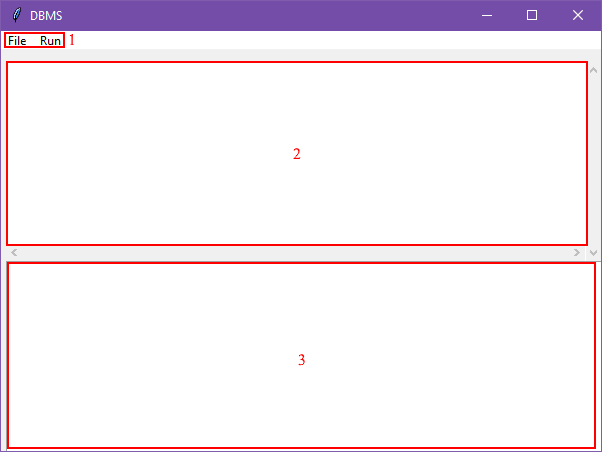
\includegraphics[width=1\linewidth]{images/interface}
	\caption{Макет рабочего окна программы}
	\label{fig:interface}
\end{figure}

Макет содержит следующие элементы:
\begin{enumerate}
	\item Главное меню
	
	Главное меню реализовано на основе виджета tk.Menu и состоит из двух основных разделов:
	\begin{itemize}
		\item File — содержит команды Save и Open для сохранения и загрузки базы данных из файла;
		\item Run — команда запуска обработки пользовательского ввода, выполняющей анализ текста, введённого в поле SQL-команды, и выполнение соответствующих операций.
	\end{itemize}
	Меню охватывает основные действия, необходимые для работы пользователя с базой данных, и остаётся доступным вне зависимости от текущего состояния приложения.
	
	\item Область отображения таблиц
	
	Эта часть интерфейса занимает верхнюю половину окна и реализована с помощью контейнера tk.Frame и виджета ttk.Treeview, предназначенного для отображения табличных структур в виде древовидной таблицы с колонками. Таблица автоматически подстраивается под содержимое и заполняет всё доступное пространство. Для удобства просмотра добавлены горизонтальная и вертикальная полосы прокрутки.
	
	При проведении операций над данными интерфейс обновляется динамически, подставляя актуальные данные в таблицу.
	
	\item Поле ввода команд
	
	В нижней части окна находится текстовое поле tk.Text, предназначенное для ввода пользователем команд на SQL-подобном языке. Это основная точка взаимодействия между пользователем и логическим ядром программы.
	
	По нажатию пункта Run введённая команда передаётся в модуль парсинга и обрабатывается соответствующим образом. Результат отображается либо в таблице, либо во всплывающем сообщении.
\end{enumerate}

Таким образом, интерфейс приложения предоставляет все необходимые средства для взаимодействия с табличными данными и служит оболочкой для логического ядра программы, выполняющего интерпретацию команд и управление данными.